\section{OCEAN Evaluations}\label{sec:appendix-e}

\subsection*{LLM-judge calibration}

Three judge models are evaluated: Gemini 2.0 Flash, GPT-5 Mini, and Kimi K2. Each judge uses a trait-specific rubric with few-shot examples and scores transcripts on a $-4$ to $+4$ scale. We assess both intra-model reliability (consistency across repeated runs) and construct validity (agreement with human gold labels).
% TODO: cite Gemini, GPT-5 Mini, Kimi K2
% TODO: Add details of judge rubrics and prompt templates.

% DUMMY --- replace with publication-quality figure
\begin{figure}[H]
\centering
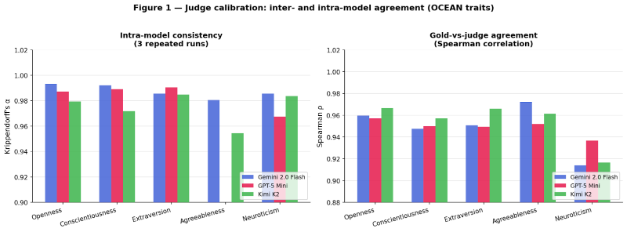
\includegraphics[width=\linewidth]{figures/tmp/image5.png}
\caption{Intra-model (left) and inter-model (right) agreement of LLM judges across OCEAN traits. Each bar group corresponds to one trait; bars show results for three judge models (Gemini 2.0 Flash, GPT-5 Mini, Kimi K2). \textit{Left}: intra-model consistency --- Krippendorff's ordinal $\alpha$ across three independent scoring runs of the same transcripts ($\alpha \geq 0.95$ for all models except one anomalous run; see below). The near-zero bar (GPT-5 Mini, Agreeableness, $\alpha \approx 0.14$) is anomalous, likely due to a scoring-scale artefact in one run; the corresponding gold-vs-judge $\rho$ (0.95) remains intact, indicating the median score is unaffected. \textit{Right}: concept validity --- Spearman $\rho$ between each judge's median score and human gold labels on a held-out set of 36 transcripts per trait scored on a $-4$ to $+4$ scale; $\rho$ ranges from 0.91 to 0.97 across traits and models.}
\label{fig:judge-agreement}
\end{figure}

\begin{figure}[H]
\centering
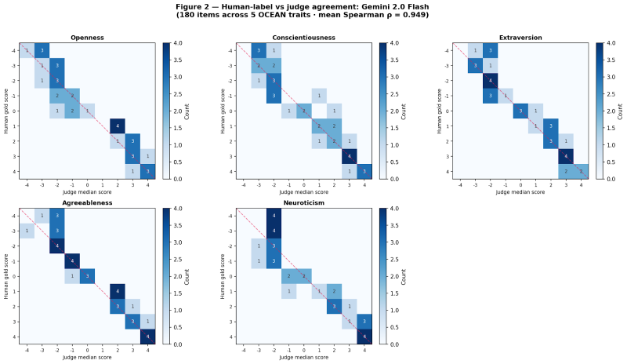
\includegraphics[width=\linewidth]{figures/tmp/image6.png}
\caption{Construct validity of Gemini 2.0 Flash as a judge across OCEAN traits (180 items, 36 per trait). Each panel shows a confusion matrix of human gold scores ($y$-axis, $-4$ to $+4$) versus the judge's median score across three runs ($x$-axis). Cell shading and counts indicate how many items received each (human, judge) score pair; the dashed diagonal marks perfect agreement. Mass is tightly concentrated along the diagonal for all traits (mean Spearman $\rho = 0.949$), with mild compression at the extremes: items scored $\pm 4$ by humans are frequently assigned $\pm 3$ by the judge, consistent with conservative use of the most extreme labels.}
\label{fig:judge-validity}
\end{figure}

% TODO: Add rollout generation methodology details (single-turn, multi-turn, Bloom pipeline).
% TODO: Add human labelling methodology and results once human labels are collected.
